\documentclass[11pt,lineno]{../style}



\newcommand{\autor}{North (1990) }

\title{
\large{Nova Economia Institucional}\vspace{2pt}\\
\Huge{\autor - \textit{Institutions, Institutional change and Economic Performance}}
}
\date{22 de Maio de 2020}

\author[$\ast$]{Gabriel Petrini}

\affil[$\ast$]{PhD Student at Unicamp.}

\keywords{
	Keyword1\\ 
	Keyword2\\
	Keyword3
}

\runningtitle{Resenha} % For use in the footer 

%% For the footnote.
\runningauthor{Petrini}

\begin{abstract}

\end{abstract}

\begin{document}

\maketitle
\marginmark
\thispagestyle{firststyle}
% Please add here a significance statement to explain the relevance of your work

\section{Introdução às instituições e à mudança institucional}

\autor abre o capítulo definindo instituições como as regras do jogo, ou ainda, como restrições humanamente concebidas que moldam a interação humana. Em seguida afirma que mudanças institucionais determinam a forma que as sociedade evoluem ao longo do tempo e, portanto, são centrais para compreender a mudança histórica. Além disso, pontua que não existe um constructo teórico que integra uma análise institucional na teoria e na história econômica.

\subsection{I}

De modo geral, as instituições diminuem a incerteza ao prover uma estrutura a vida cotidiana e por guiar as interações humanas. Em seguida, categoria instituições em formais e informais em que regras são exemplos das primeira enquanto convenções e códigos de conduta são exemplos da segunda. Também destaca que as instituições podem ser criadas e evoluir ao longo do tempo. Pontua a dimensão negativa (restrição de ações) quanto positiva (permissividades) das instituições, ou seja, envolvem as interações humanas. Adiante, diferencia instituições de \textbf{organizações} em que as segundas surgem como consequência do --- e influenciam o --- arranjo institucional e incluem grupos políticos, econômicos, sociais e educacionais em que tais agrupamentos possuem objetivos em comum.
Outra distinção relevante é entre agentes e as regras/normas (jogadores das regras).

Adiante, \autor discute que as instituições são criadas e alteradas pelos humanos de modo a teoria institucional que propõe deve partir do \textbf{nível individual}.
Também pontua que as instituições determinam o desempenho econômico ao afetar os custos de produção.

\subsection{II}

Mais uma vez, o autor retoma que instituições reduzem as incertezas de uma sociedade ao promover uma estrutura estável às interações humanas, mas tal estabilidade não implica imutabilidade. Argumenta que as mudanças institucionais são complexas uma vez que podem ser consequências de mudanças formais, informais e nas formas de execução. Pontuam que as instituições informais estão menos sujeitas à ações políticas do que as formais. Dito isso, direciona a discussão para as condições que levam a uma maior convergência ou divergência das sociedades\footnote{Afirma que abandonou a explicação via incentivos de preços antes defendida em outro livro.}. Defende que a resposta a esse questão se dá pela interação entre instituições e organizações assim como na determinação de oportunidades associadas ao arranjo institucional em que as organizações são criadas para extrair vantagens dessas oportunidades e, na medida que se altera, modificam as instituições. 

Argumenta que a trajetória da mudança institucional é determinado pelo \textit{lock-in} derivado da relação entre instituições e organizações e pelos \textit{feedbacks} dos agentes. Destaca ainda que as mudanças institucionais (incrementais) decorrem da percepção dos agentes das organizações políticas e econômicas podem ser favorecidos ao alterar o arranjo institucional na margem. No entanto, esta percepção depende da obtenção e processamento dessas informações. Em seguida, destaca que custos de transação (políticos e econômicos) tornam os \textbf{direitos de propriedade} ineficientes, mas a racionalidade limitada dos agentes tornam tais direitos de propriedade persistentes.

\autor afirma também que as mudanças institucionais podem tanto melhorar quanto piorar o bem-estar econômico. À luz disso, defende que o sucesso da economia norte-americana decorre pelo arranjo institucional gerar --- em média --- efeitos positivos sobre a atividade produtiva (apesar de suas consequências adversas). Ao mesmo tempo, afirma que o insucesso dos países do ``Terceiro Mundo'' decorrem do favorecimento de atividades redistributivas invés de produtivas, restringindo oportunidades invés de ampliá-las uma vez que as organizações oriundas deste arranjo institucional são mais eficientes em tornar esta sociedade mais improdutiva. Argumenta que esta trajetória se torna persistente por conta dos custos tando do mercado econômico quanto do político que se soma aos modelos subjetivos dos agentes de modo que não mudam em direção mudanças (incrementais) mais eficientes.
\section{Cooperação: o problema teórico}

\autor abre o capítulo pontuando que a teoria neoclássica não apenas deixa de conceituar diferente organizações de troca (que não mercado) como também não explica a persistência de organizações ``ineficientes'' ao longo do tempo. No entanto, afirma que tal teoria não discute tais temas uma vez que partem da hipótese de que os direitos de propriedade são bem definidos (a um custo desprezível) e que a informação está disponível (também a um custo baixo). Em linhas gerais, o autor argumenta que a teoria neoclássica carece de uma melhor compreensão da \textbf{coordenação e cooperação} dos agentes econômicos. Além disso, enfatiza a importância dos \textbf{custos de transação e das instituições}.

\subsection{I}

Por mais que os economistas --- de modo geral --- tenho demorado para levar em consideração a importância das instituições, já vem de um tradição que explora os problemas de coordenação e o fazem por meio do arcabouço da \textbf{teoria dos jogos}. Em seguida, \autor pontua que a cooperação não é sustentável nas configurações mais próximas da realidade, ou seja, quando os jogos não são repetitivos; quando a informação não é completa e; quando existe um grande número de jogadores. Adiante, discute alguns avanços da literatura e coloca:

\begin{quotation}
	[U]nder what conditions can voluntary cooperation exist without the Hobbesian solu­tion of the imposition of a coercive state to create cooperative solutions? [...] We do not observe political anarchy in high-income countries. On the other hand the coercive power of the state has been employed throughout most of history in ways that have been inimicable to economic growth (North, 1981, Chapter 3).
	But it is difficult to sustain complex exchange without a third party to
	enforce agreements.
\end{quotation}
Em seguida, \autor explicita aquilo que considera o centro da análise das comunidades, convenções e da cooperação: qual o mínimo que é preciso saber sobre os demais agentes de modo a formar noções de seu comportamento e, com isso, ser capaz de interagir com eles?

\subsection{II}

O autor abre a seção afirmando que a competição elimina os problemas da informação completa e assimétrica. No entanto, para isso é preciso supor configurações institucionais e informacionais muito estringentes. Além disso, a teoria-padrão não apenas pressupõe que os agentes possuem objetivos bem definidos, mas que sabem as escolhas corretas para obtê-los. Outra limitação surge na presença de elevados custos de transação em que supõe-se que as instituições são desenvolvidas para gerar resultados eficientes e que independem do desempenho econômico.

Em linhas gerais, \autor afirma que nenhumas dessas condições extremas são observadas uma vez que os agentes econômicos atuam com informações incompletas a partir de modelos subjetivos e potencialmente errados cuja informação não é suficiente para corrigí-los. Além disso, instituições são criadas para servir aos interesses daqueles que possuem maior poder de barganha, ou seja, não são desenvolvidas necessariamente para serem eficientes. Em um mundo em que os custos de transação são desprezíveis, prossegue, este poder de barganha não é tão relevante, mas como este não é o caso, o poder de barganha afeta as instituições e, por conseguinte, o desempenho econômico:

\begin{quotation}
	If economies realize the gains from trade by creating relatively efficient
 institutions, it is because under certain circumstance5 the private objec­tives of those with the bargaining strength to alter institutions produce institutional solutions that turn out to be or evolve into socially efficient ones. The subjective models of the actors, the effectiveness of the institu­tions at reducing transaction costs, and the degree to which the institu­tions are malleable and respond to changing preferences and relative prices determine those circumstances.
\end{quotation}

\section*{Capítulo 03: Governança de relações contratuais}

Em linhas gerais, ECT estabelece que a variedade de instituições está associada com os atributos das \textbf{transações} e que o propósito de eficiência das instituições diz respeito à combinação da estrutura de governança adequada aos atributos mencionados. Dito isso, neste capítulo, Williamson analisa as diferentes teorias e abordagens dos contratos.

\subsection*{Tradições contratuais}

O autor argumenta que o paradigma da \textbf{transação discreta} é difundido tanto em direito quanto em economia, mas há o reconhecimento que muitas relações contratuais não podem ser configuradas enquanto discretas.

\begin{description}
	\item[Clássica] Enfatiza o caráter discreto e presencial (``\textit{presentation}'') dos contratos. Implica irrelevância das partes contratuais e destaca em regras formas;
	\item[Neo-clássica] Parte do reconhecimento de que o mundo é um sistema complexo e que os contratos são incompletos por consequência e que as partes irão cumpri-los a depender da confiança no aparato jurídico associado;
	\item[Relacional] A impessoalidade da teoria clássica é descartada e dá lugar a um tratamento relacional ao longo do tempo em que a especificidade das transações se destacam
\end{description}


\begin{figure}[h]
	\centering
	\caption{Transações ilustrativas}
	\label{fig:screenshot006}
	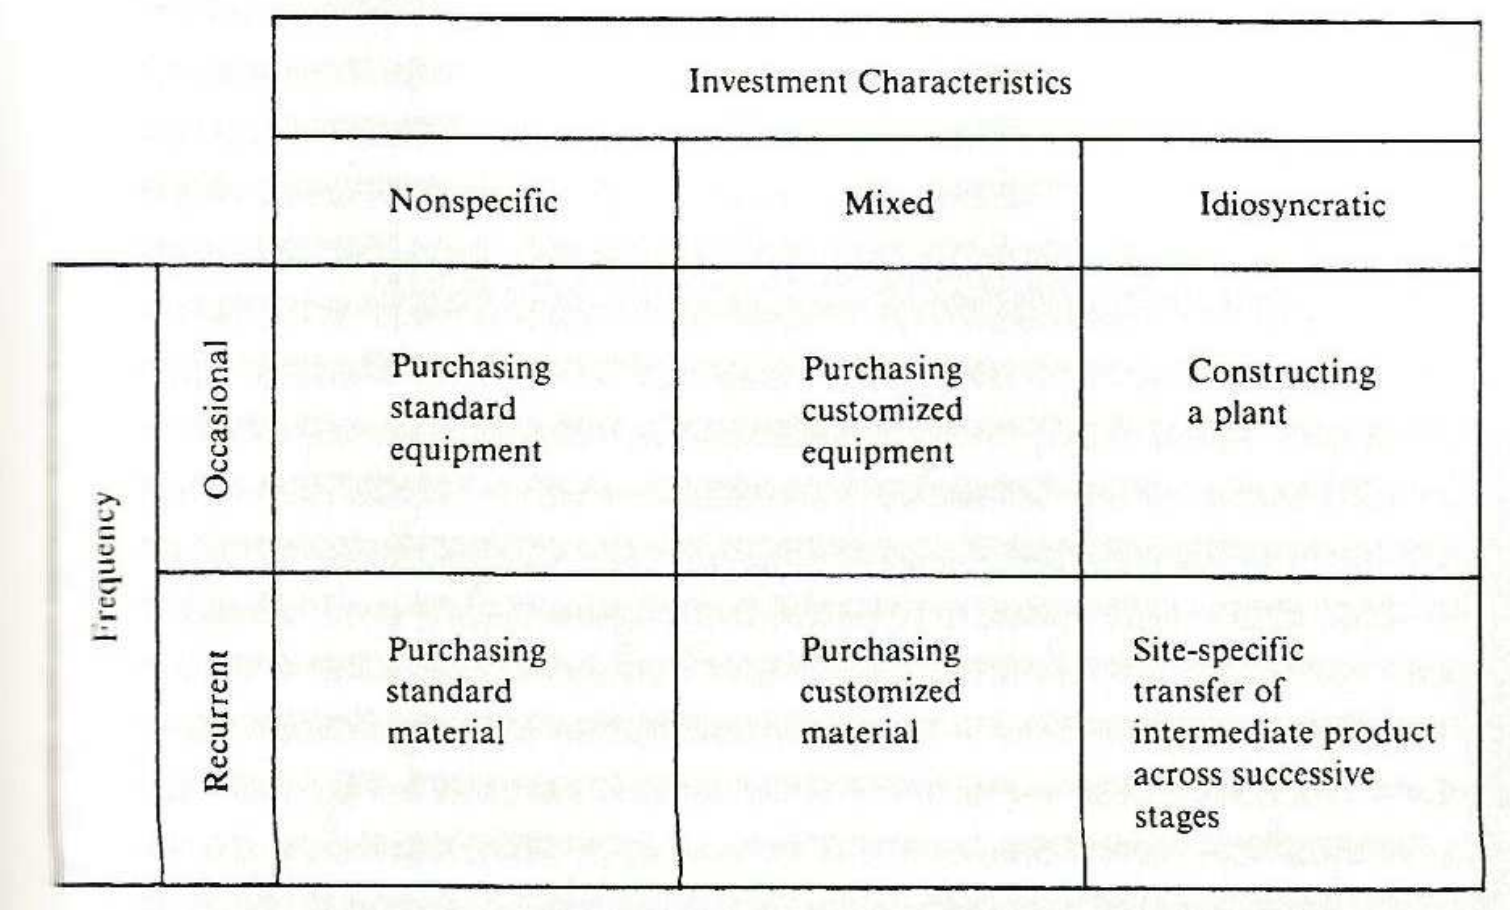
\includegraphics[width=0.7\linewidth]{screenshot006}
\end{figure}



\subsection*{Governanças eficientes}

Apesar das transações terem outras dimensões, Williamson irá focar na especificidade dos ativos e na frequência categorizados da seguinte maneira e sintetizados na tabela abaixo:

\begin{itemize}
	\item Frequência
	\begin{itemize}
		\item Única
		\item Ocasional
		\item Recorrente
	\end{itemize}
	\item Especificidade dos ativos
	\begin{itemize}
		\item Não-específicos
		\item Mistos
		\item Altamente específicos
	\end{itemize}
	\item Hipóteses simplificadoras
	\begin{itemize}
		\item Firmas temporárias podem ser desconsideradas
		\item Ofertantes potenciais são numerosos
		\item Frequência diz respeito à atividade de compra no mercado somente
		\item $\therefore$ Apenas transações ocasionais e frequentes serão consideradas e a especificidade da governança está diretamente associada tanto com a frequência quanto com a especificidade do ativo em questão
	\end{itemize}
\end{itemize}

\begin{figure}[h]
	\centering
	\caption{Governanças eficientes}
	\label{fig:screenshot007}
	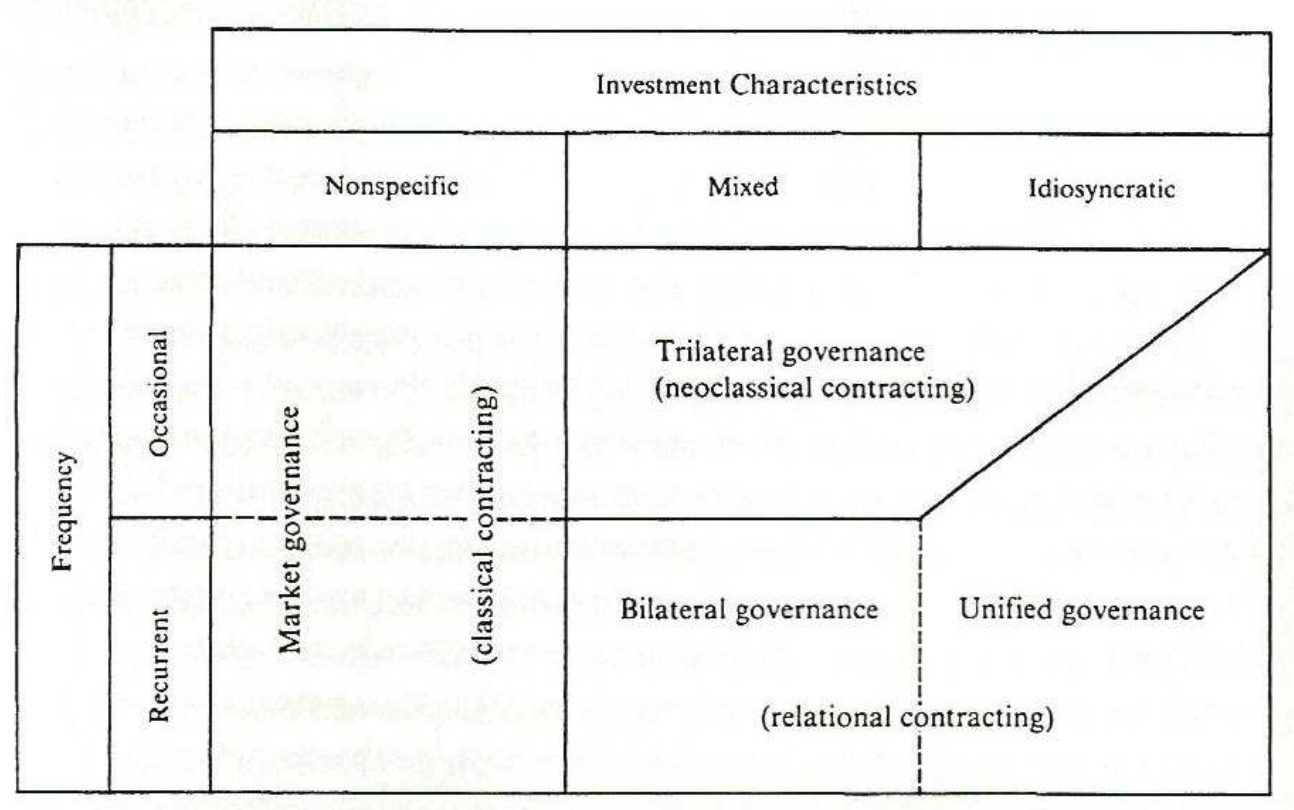
\includegraphics[width=0.7\linewidth]{screenshot007}
\end{figure}




\begin{description}
	\item[Mercado:] É a principal estrutura de governança para transações \textbf{não-específicas}, sejam elas ocasionais ou frequentes. Este tipo de transação é aquele que os contratantes estão menos aptos a se basear em suas experiências para estabelecer salvaguardar contra o comportamento oportunista. Em linhas gerais, as implicações do paradigma discreto se aplicam a esta estrutura de governança. A identidade das partes é negligenciável e o conteúdo das transações está sujeito à formalidades;
	\item[Trilateral:] São mais necessárias em transações ocasionais em que a especificidade é mista ou elevada. Sendo assim, não existem incentivos suficientes para que o contrato se dê via competição, ou seja, o mercado é insuficiente.
	\item[Bilateral:] São mais frequentes em transações frequentes cuja especificidade dos ativos é média ou elevada. Como consequência, a \textbf{transformação fundamental} ocorre por conta da natureza não convencional/padronizada das transações. Além disso, a recorrência das transações faz com que os custos elevados de uma governança especializada seja diluído. Além disso, tais estruturas preservam a \textbf{autonomia} das partes, seja pela verticalização ou relação entre-firmas. Ambas as partes têm incentivos para preservas as relações contratuais.
	\item[Unificada:] Os incentivos para as relações entre-firmas se reduzem na medida que as transações se tornam progressivamente mais específicas, ou seja, menos transferível para o uso de outros sem perdas significativas de modo que as economias de escala são realizadas por uma das partes (verticalização). A vantagem da verticalização é a menor necessidade de revisão dos contratos entre-firmas.
\end{description}

\subsection*{Incerteza}

A presença da incerteza impõe uma problema adaptativo e sequencial. Em linhas gerais, um maior grau de incerteza não afeta significativamente as transações de ativos menos específicos. No entanto, quanto maior a \textbf{especificidade dos ativos} e dada a necessidade de \textbf{continuidade} das relações contratuais, a incerteza se torna mais impositiva de modo que estruturas de governança mais adequadas são necessárias. Uma forma de lidar com a incerteza é optar por ativos menos específicos e mais usuais de modo que a governança de mercado é mais adequada. No entanto, tal especificidade pode ser preservada com uma forma de organização internalizada.

\subsection*{Mensuração}

Em linhas gerais, Williamson pontua que os problemas de governança e mensuração (ambos ramos da ECT) são negligenciáveis na ausência \textbf{tanto} de racionalidade ilimitada \textbf{quanto} de comportamento oportunista. Na ausência de racionalidade limitada, os custos de mensuração são nulos em que o comportamento oportunista invalidado. Na ausência de comportamento oportunista, a incompletude dos contratos deixa de ser um problema de governança.


\subsection*{Distribuição das transações}

Nesta seção, Williamson discute qual a ``distribuição de frequência'' dos diferentes tipos de contrato e transações. Conclui que uma distribuição \textbf{uniforme} é a que melhor descreve o mundo contratual.
\section{Teoria de troca com custos de transação}

Neste capítulo, \autor adiciona uma \textbf{teoria da produção} às hipóteses comportamentais discutidas anteriormente. Por custos de produção, considera tanto os custos de transformação quanto os de transação. O custo por se obter \textbf{informações} é o principal elemento dos custos de transação e consiste na \textbf{mensuração dos valores dos atributos} dos ativos e inclui o que está sendo transacionado; os custos de proteção dos direitos de propriedade e policiamento e; execução contratual. Em linhas gerais, argumenta que a mensuração e os custos de execução são os determinantes sociais, políticos e econômicos das instituições.

\subsection{I}

\autor pontua que os autores da teoria dos CT não têm se debruçado a entender o que tornais tais custos tão \textbf{elevados} e que esta é uma questão central em sua teoria. Resumidamente, uma troca gera custos associados à tentativa de mensurar o valor dos atributos desses ativos. Dentre os elementos que explicam o porquê que tais custos de mensuração são elevados, desta a assimetria de informação.

\subsection{II}

O autor inicia esta seção discutindo o modelo Walrasiano básico em que preços são mecanismos alocativos suficientes para determinar os valores de uso. A esse modelo, o autor soma os custos de informação e, assim, os ganhos líquidos devem considerar os custos de mensuração e de policiamento dos acordos. Uma vez que a mensuração de tais atributos é custosa, a renda capturada por meio da obtenção de informação se torna mais importante. Além disso, a maximização do valor de um ativo envolve uma estrutura de propriedade na qual as partes que podem influenciar a variabilidade de atributos específicos tornam-se requerentes residuais sobre esses atributos.

\subsection{III}

Uma vez que não se sabe os atributos de um bem ou serviço, assim como o desempenho de uma das partes e porque é necessário destinar recursos para obter e medir e monitorar tais características é que surgem questões de execução. Tal execução pode vir tanto da retaliação de uma das partes como também dos códigos de conduta internos ou de um terceiro ente de forma coercitiva (Estado). De todo modo, a execução não pode ser tomada como garantida e a dificuldade aumenta na medida que a divisão do trabalho também aumenta. Em seguida, afirma:

\begin{quotation}
	But without institutional con­straints, self-interested behavior will foreclose complex exchange, be­cause of the uncertainty that the other party will find it in his or her interest to live up to the agreement. The transaction cost will reflect the uncenainty by including a risk premium, the magnitude of which will turn on the likelihood of defection by the other party and the consequent cost to the first party. 
\end{quotation}

\subsection{IV}

\autor argumenta que a apropriação --- que é importante para a definição dos direitos de propriedade --- é função das regras legais, das formas organizacionais, execução e normas comportamentais. Em resumo, a apropriação depende do arranjo institucional. Uma vez que os custos de transação existem na presença de direitos de propriedade, tais direitos nunca são perfeitamente especificados ou executados. Além disso, pelos custos de transação terem mudado consideravelmente ao longo do tempo, as configurações de formas de proteção ou de captura dos direitos de propriedade também variam enormemente. Sendo assim, as instituições determinam a estrutura das trocas que, por sua vez, determinam os custos de produção (transformação e transação). As instituições são mais eficazes em resolver questões de coordenação e produção a depender da motivação dos agentes, a complexidade do ambiente e a capacidade dos agentes de decifrá-la. Dito isso, o autor pontua que os custos de transação aumentam com o grau de complexidade da economia, ou seja, são menores em uma economia de pequena escala e de transação local e conclui:

\begin{quotation}
	Thus, it should be readily apparent that to devcJop a model
	of institu­tions, we must explore in depth the structural characteristics of informal constraints, formal rules, and enforcement and the way in which they evolve. Then we shall be in a position to put them together to look at the overall institutional makeup of political/economic orders.
	
\end{quotation}

	
\begin{redbox}{Dúvidas e comentários}	
	Seria a teoria institucional de North uma ``Teoria Geral das Instituições'' em que a teoria neoclássica é um caso especial? Em outras palavras, North tenta estender/compatibilizar suas contribuições com a teoria \textit{mainstream} ou romper com ela? \textbf{Comentário:} Williamson me pareceu menos preocupado com essa compatibilização com a teoria-padrão.
\end{redbox}

\end{document}
